\subsection{Herstellung der Compact Disc mittels des Spritzgussverfahrens}
\label{subsec:cdherstellung}

Die Herstellung einer CD beginnt mit der Anfertigung einer Glasmatrize, die aus
einer Glasplatte und einer Fotolackschicht besteht, welche die Pitstruktur
enthält. Aus der Glasmatrize wird eine Metallmatrize gefertigt, welche für das
Spritzgussverfahren verwendet wird. Dabei wird die Matrize in das flüssige
Polycarbonat gepresst, wodurch die Pitstruktur auf die Polycarbonatscheibe
übertragen wird (siehe \autoref{fig:cdherstellung}). Auf diese wird anschließend
das Aluminium aufgedampft, um die Reflexionsschicht zu erhalten. Im letzten
Schritt wird die Reflexionsschicht mithilfe einer Schutzschicht versiegelt.
\cite{cdp}

\begin{figure}[h]
    \begin{center}
        \begin{minipage}[t]{\textwidth}
            \begin{center}
                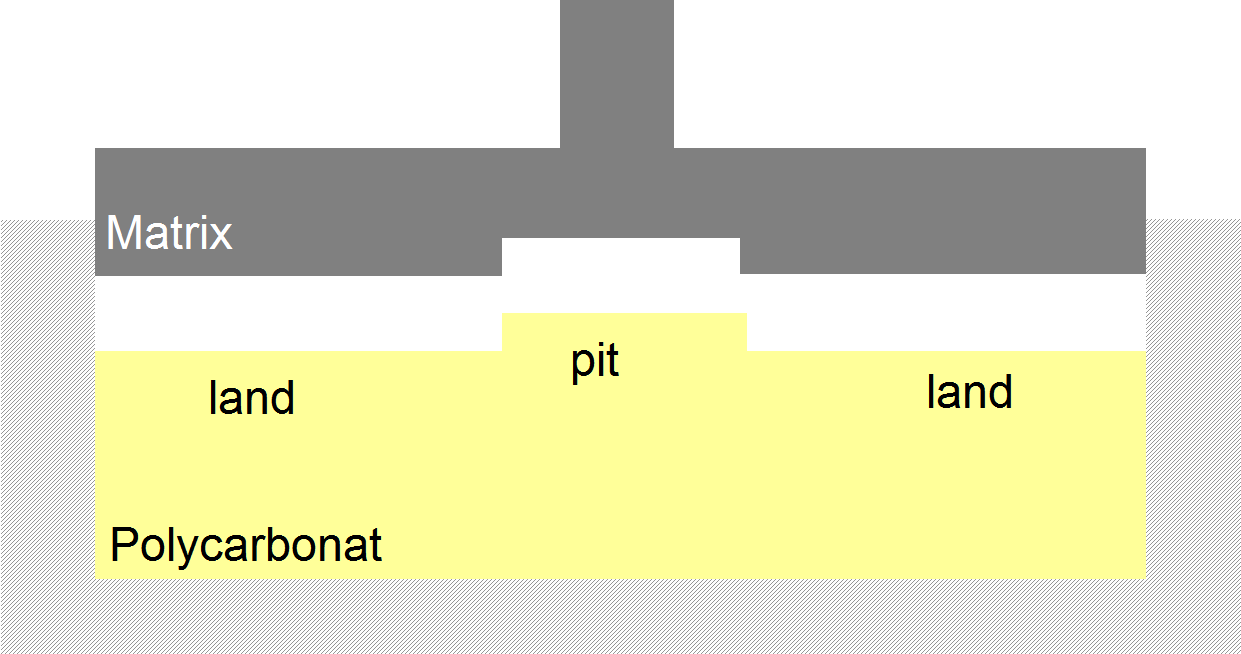
\includegraphics[height=0.1\textheight]{Bilder/Optische_Datentraeger_Die_Compact_Disc/Herstellung/cdherstellung.png}
                \caption[Übertragung der Pitstruktur \newline \url{http://daten.didaktikchemie.uni-bayreuth.de/umat/cd_dvd/spritzguss.gif} (zuletzt aufgerufen am 07.08.2015)]{Übertragung der Pitstruktur}
                \label{fig:cdherstellung}
            \end{center}
        \end{minipage}
    \end{center}
\end{figure}

Das Spritzgussverfahren selbst unterteilt sich in drei Schritte. Wie in
\autoref{fig:cdspritz} zu sehen ist, wird zunächst zerkleinertes Polycarbonat
(Granulat) in die Schnecke eingefüllt. Durch die Heizelemente und die sich
drehende Schnecke verflüssigt sich das Granulat. Der an der Spitze sich
aufbauende Druck presst die Schnecke teilweise aus dem Gehäuse
(Plastifizierzylinder). Diesen Schritt nennt man Plastifizieren. Danach folgt
der Einspritzvorgang. Dabei wird das geschmolzene Granulat durch die
Vorwärtsbewegung der Schnecke in die CD-Form und auf die Matrize gedrückt. Nach
dem Abkühlen wird die fertige Polycarbonatscheibe ausgeworfen. \cite{cdpf}

\begin{figure}[h]
    \begin{center}
        \begin{minipage}[t]{\textwidth}
            \begin{center}
                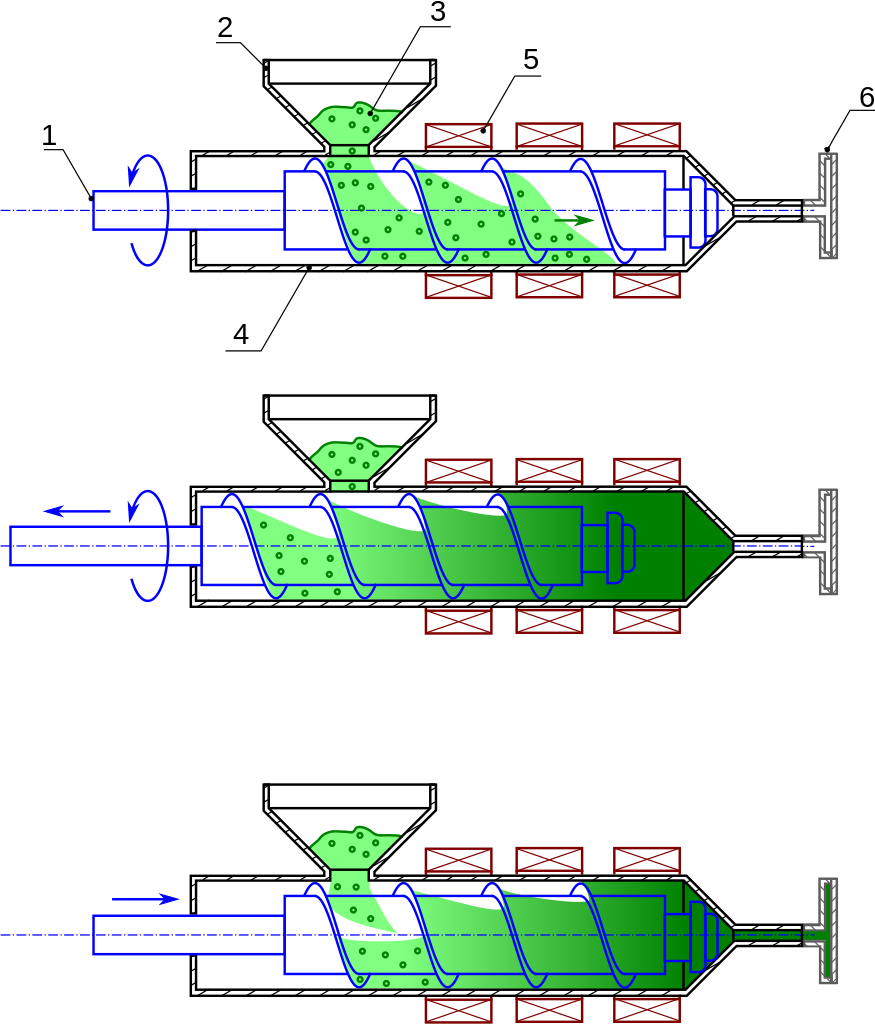
\includegraphics[height=0.5\textheight]{Bilder/Optische_Datentraeger_Die_Compact_Disc/Herstellung/cdspritz.png}
                \caption[Spritzgussverfahren \newline \url{https://upload.wikimedia.org/wikipedia/commons/thumb/2/23/Principe_moulage_injection_polymere.svg/899px-Principe_moulage_injection_polymere.svg.png} (zuletzt aufgerufen am 11.08.2015)]{Spritzgussverfahren: 1. Schnecke, 2. Einfülltrichter, 3. Granulat, 4. Plastifizierzylinder, 5. Heizelemente, 6. CD-Form inklusive Glasmatrize}
                \label{fig:cdspritz}
            \end{center}
        \end{minipage}
    \end{center}
\end{figure}
